\documentclass[11pt]{article}

\usepackage[utf8]{inputenc}
\usepackage[T1]{fontenc}
\usepackage[french]{babel}
\usepackage[margin=1in]{geometry}
\usepackage{amsmath}
\usepackage{amssymb}
\usepackage{graphicx}
\graphicspath{{../}}
\usepackage{hyperref}
\usepackage{xcolor}
\usepackage{enumitem}
\usepackage{float}
\usepackage{tikz}
\usetikzlibrary{arrows.meta, positioning}

\hypersetup{
  colorlinks=true,
  linkcolor=blue!50!black,
  citecolor=blue!50!black,
  urlcolor=blue!50!black,
  pdftitle={Ce que signifie la vraisemblance},
  pdfauthor={Warith Harchaoui}
}

\usepackage[round]{natbib}
\bibliographystyle{plainnat}

\newcommand{\code}[1]{\texttt{#1}}

\title{Ce que signifie la vraisemblance~: \\ d'un produit brut à un score borné et comparable}
\author{Warith Harchaoui}
\date{Été 2026}

\begin{document}
\maketitle

\begin{abstract}
Cette note dérive, à partir des principes de base, une seule idée
utilisée à travers la statistique, la théorie de l'information et
l'apprentissage automatique~: lire la vraisemblance non comme le
produit brut par lequel tout traité classique commence, mais comme une
\emph{moyenne} exponentiée de log-densités, $L := \exp(\mathbb E[\ln
p])$. Cette reformulation est inhabituelle~: presque aucune référence
classique ne définit la vraisemblance ainsi. Cette note explique
précisément pourquoi elle se justifie~: une identité exacte qui la
relie au produit classique, une lecture directe en théorie de
l'information (inégalité de Jensen, entropie de Shannon, un
raffinement indexé par une température emprunté à la mécanique
statistique à l'équilibre), deux résultats asymptotiques classiques
(les grandes déviations de Cram\'er et la martingale de Wald) qui
décrivent exactement le comportement à long terme de cette quantité,
et un compte rendu précis de $L$ comme estimateur statistique, biais et
variance compris, ainsi qu'une preuve que le produit brut qu'il
remplace n'estime rien de fixe du tout. Deux cas travaillés, un modèle
de classification catégorielle et un modèle de régression sous bruit
gaussien, montrent la même construction retomber sur l'inverse d'une
mesure d'erreur familière dans les deux cas, la perplexité dans le
premier, l'erreur quadratique moyenne racine dans le second. La propre
note de mathématiques d'\code{elbow-helper}, \code{ELBOW-fr.tex},
construit ses critères de sélection de modèle gaussiens (BIC, mBIC,
ICL) sur le socle dérivé ici plutôt que de le rederiver. Les citations
suivent la même convention de sourçage que \code{ELBOW-fr.tex}~: chaque
affirmation précise s'il s'agit d'une citation vérifiée, d'une citation
rapportée par une source secondaire, ou d'une construction propre à
cette note.
\end{abstract}

\clearpage

\tableofcontents

\clearpage

\section{La notion}
\label{sec:notion}

Les données désignent ici $n$ paires $(x_i, y_i)$, une entrée $x_i$
associée à un résultat $y_i$~: une covariable pilotant une prédiction,
une position pilotant la hauteur d'une courbe, ou rien du tout, $x_i$
simplement absent, pour un modèle qui ne décrit jamais que $y_i$ seul.
Un unique modèle graphique couvre chaque cas que cette note utilise,
$\theta$ et $x_i$ alimentant une densité conditionnelle qui engendre
$y_i$~:

\begin{center}
\begin{tikzpicture}[
  node distance=13mm and 16mm,
  box/.style={draw, rounded corners, minimum height=8mm, minimum width=25mm,
    align=center, font=\small, fill=blue!4},
  ->, >=Stealth, thick
]
\node[box] (theta) {$\theta$};
\node[box, right=of theta] (dens) {$p(\cdot \mid x_i,\theta)$};
\node[box, right=of dens] (y) {$y_i$};
\node[box, below=of dens, fill=red!4] (x) {$x_i$};
\draw (theta) -- (dens);
\draw (dens) -- (y);
\draw (x) -- (dens);
\end{tikzpicture}
\end{center}

La \emph{vraisemblance} désigne la densité jointe des résultats
observés, lue comme une fonction du paramètre plutôt que des
données~: $L_{\text{brute}}(\theta) := \prod_{i=1}^n p(y_i \mid x_i,
\theta)$, un simple produit de $n$ termes, un par observation. C'est la
définition par laquelle tout traité classique commence, celle de
Bishop parmi les plus claires \citep{bishop2006prml}. C'est aussi
exactement la quantité qu'un facteur de Bayes ou un test du rapport de
vraisemblance de Neyman-Pearson compare directement. Laissée sous
forme de produit brut, c'est pourtant un mauvais matériau pour
construire un score borné~: $n$ densités multipliées entre elles
finissent soit par s'écraser vers zéro soit par exploser à mesure que
$n$ grandit, si bien que $L_{\text{brute}}$ sur $40$ points et
$L_{\text{brute}}$ sur $4\,000$ points ne sont pas des nombres qu'un
même seuil pourrait jamais comparer~; le produit brut porte la taille
de l'échantillon dans sa propre échelle.

Cette note s'écarte de cette convention dès maintenant et le dit
franchement plutôt que de laisser cet écart implicite dans une
formule~: elle prend la vraisemblance \emph{par observation} dès le
départ, une moyenne \emph{exponentiée} de log-densités plutôt qu'un
produit brut,
$$L := \exp\!\big(\mathbb E[\ln p]\big) = L_{\text{brute}}^{\,1/n},$$
la moyenne géométrique des $n$ densités individuelles, exactement la
racine $n$-ième de $L_{\text{brute}}$, jamais un nombre différent, une
forme différente du même nombre seulement. Presque aucune référence
classique ne définit la vraisemblance ainsi. La raison n'est pas
stylistique~: diviser la somme de l'exposant par $n$ avant de
réexponentier est exactement ce qui transforme une quantité extensive,
dont l'échelle dépend de la taille de l'échantillon, en une quantité
intensive, dont l'échelle n'en dépend pas, le même geste que fait la
théorie de l'information quand elle travaille avec la
\emph{perplexité}, une \emph{moyenne} exponentiée de log-probabilité
plutôt qu'une probabilité jointe brute (rendu explicite à la
section~\ref{sec:cas}).

\section{Ce que le nombre signifie}
\label{sec:sens}

Avant toute machinerie asymptotique, $L$ a une lecture directe qui
mérite qu'on s'y arrête. Par l'inégalité de Jensen, $\ln$ étant
concave, $L = \exp(\mathbb E[\ln p]) \le \mathbb E[p]$ toujours~: la
moyenne géométrique sur laquelle repose cette note ne dépasse jamais
la moyenne arithmétique de ces mêmes densités, avec égalité seulement
quand $p$ est constante sur les observations.

Pour un $p$ discret sur $K$ catégories, prenons l'espérance sous $p$
lui-même plutôt que sous les données~: $\exp(\mathbb E_{y \sim p}[\ln
p_y]) = \exp(-H(p))$, l'entropie de Shannon \citep{mackay2003information}
lue comme une probabilité plutôt que comme un compte de bits. Cela
reste dans $[1/K, 1]$~: égal à $1/K$ quand $p$ est uniforme sur les
$K$ catégories, montant vers $1$ à mesure que $p$ se concentre sur
l'une d'elles. Lue ainsi, $\exp(-H(p))$ est une probabilité typique, ou
effective. Son inverse $\exp(H(p))$ est le nombre effectif de
catégories plausibles~: $\exp(H(p)) \approx 4$ signifie une incertitude
comparable à un choix équiprobable parmi quatre.

\textbf{Une lecture en température.} Cette borne admet un raffinement à
un paramètre qui mérite d'être rendu précis plutôt que simplement
évocateur. Pour $\beta > 0$, définissons la famille inclinée par
puissance $p_\beta(y) := p(y)^\beta / Z(\beta)$, $Z(\beta) := \int
p(y)^\beta\,dy$ (ou $\sum_y p(y)^\beta$ dans le cas discret)~: une
véritable famille exponentielle, où $\beta$ joue le rôle que Gibbs
attribue à la température inverse face à l'« énergie » $-\ln p(y)$.
C'est exactement l'objet que décrit le dictionnaire grandes
déviations~/~mécanique statistique~: $\ln Z(\beta)$ est une énergie
libre mise à l'échelle, $\beta$ sa température inverse, et la relation
de transformée de Legendre qu'utilise l'argument de Cram\'er de la
section~\ref{sec:pourquoi} pour la fonction de taux est, terme à terme,
celle qui relie énergie libre et entropie en mécanique statistique à
l'équilibre \citep{touchette2009}. Dériver en $\beta=1$, où $p_\beta =
p$, redonne $L$ lui-même~: $\frac{d}{d\beta} \ln Z(\beta)\big|_{\beta=1}
= \mathbb E_p[\ln p] = \ln L$, si bien que $L$ est une dérivée d'une
énergie libre, évaluée à une température précise. L'entropie de Shannon
ci-dessus est elle-même la limite $\beta \to 1$ de l'entropie de
R\'enyi $H_\beta(p) := \ln Z(\beta)/(1-\beta)$, un fait standard
vérifiable directement à partir des définitions ci-dessus.

Les deux extrêmes de $\beta$ se lisent exactement comme les deux
extrêmes de température, rendus précis plutôt que laissés à l'image.
Quand $\beta \to 0^+$, chaud et maximalement agité, $p_\beta$
s'aplatit vers l'uniforme sur le support de $p$ quelle que soit
l'allure de $p$ lui-même~: $Z(\beta) \to K$ dans le cas à $K$
catégories, si bien que $\exp(-H_\beta(p)) \to 1/K$, exactement le
plancher dérivé plus haut. Quand $\beta \to \infty$, froid et gelé,
$p_\beta$ s'effondre sur le mode propre de $p$~: $\exp(-H_\beta(p)) \to
\max_k p_k$, la probabilité de la catégorie la plus probable, un
plafond plus serré et dépendant de $p$ que la borne supérieure lâche
de $1$ (atteinte seulement dans la limite dégénérée où $p$ lui-même est
déjà une masse ponctuelle). Vérifié numériquement sur $p = (0{,}5,
0{,}3, 0{,}15, 0{,}05)$~: $\exp(-H_\beta(p))$ passe de $0{,}25 = 1/4$
quand $\beta \to 0$ à $0{,}5 = \max_k p_k$ quand $\beta \to \infty$, de
façon monotone, en passant par $\exp(-H(p)) \approx 0{,}32$ à $\beta =
1$. Les deux extrêmes familiers de l'eau à pression atmosphérique, le
gel à $0\,^\circ\mathrm C$ et l'ébullition à $100\,^\circ\mathrm C$,
illustrent physiquement exactement cette forme, un système fixe balayé
d'une phase ordonnée, à faible entropie, vers une phase désordonnée, à
forte entropie, à mesure qu'un paramètre analogue à une température
inverse parcourt sa plage, non une correspondance numérique~: rien ici
n'affirme que $\beta = 0$ ou $\beta = \infty$ se situent littéralement
à ces deux valeurs Celsius, seulement que le mécanisme qualitatif et sa
comptabilité exacte en transformée de Legendre sont ceux que la
mécanique statistique à l'équilibre a déjà établis.

\begin{figure}[H]
\centering
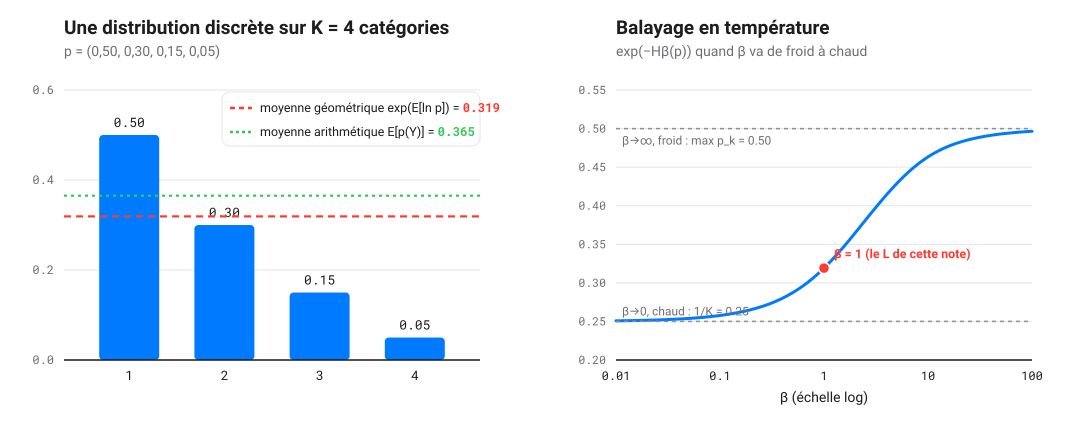
\includegraphics[width=\textwidth]{figures/temperature_sweep_fr.png}
\caption{À gauche~: le diagramme en barres ci-dessus, $p = (0{,}5,
0{,}3, 0{,}15, 0{,}05)$, avec sa moyenne géométrique $\exp(\mathbb
E[\ln p]) \approx 0{,}319$ et sa moyenne arithmétique $\mathbb E[p(Y)]
\approx 0{,}365$ marquées, l'inégalité de Jensen rendue visible par
deux lignes horizontales plutôt que laissée en simple formule. À
droite~: $\exp(-H_\beta(p))$ balayé sur $\beta$, chaud à gauche, froid
à droite, se déplaçant de façon monotone du plancher $1/K = 0{,}25$ au
plafond $\max_k p_k = 0{,}5$, avec $\beta = 1$, le $L$ propre de cette
note, marqué là où il se situe sur ce trajet.}
\label{fig:temperature}
\end{figure}

\section{Pourquoi une moyenne, pas une somme~: grandes déviations et martingales}
\label{sec:pourquoi}

Deux résultats classiques disent que ce n'est pas une simple remise à
l'échelle de confort. Notons $Z_i := \ln p(y_i \mid x_i, \theta)$ la
log-densité par observation, si bien que $L = \exp\big(\frac1n\sum_i
Z_i\big)$, une moyenne empirique exponentiée. D'abord, la relation
exacte que cela redonne avec $L_{\text{brute}}$~: $L^n =
\exp\big(\sum_i Z_i\big) = \prod_i p(y_i \mid x_i, \theta) =
L_{\text{brute}}(\theta)$. Prendre la racine $n$-ième puis
réexponentier une moyenne ne perd aucune information par rapport au
produit brut~; c'est le même nombre, à une racine $n$-ième près,
désormais exprimé sous la seule forme dont le comportement à grand
échantillon est compris.

Le théorème de Cram\'er \citep{cramer1938}, le résultat fondateur de
la théorie des grandes déviations, dit qu'une moyenne empirique
i.i.d.\ comme $\frac1n\sum_i Z_i$ fait plus que converger vers
$\mathbb E[Z]$, la garantie de la loi des grands nombres~: la
probabilité qu'elle s'écarte de cette limite de plus qu'une quantité
fixe décroît exponentiellement en $n$, à un taux fixé par une fonction
de taux convexe, la transformée de Legendre de la fonction génératrice
des cumulants de $Z$. Travailler d'abord avec la moyenne, plutôt
qu'avec le produit brut $L^n$ dont elle n'est qu'une racine $n$-ième,
expose cette structure exponentielle au lieu de l'enfouir dans un
nombre déjà multiplié.

Chernoff \citep{chernoff1952} spécialise exactement cette machinerie à
la décision entre deux densités $p_0, p_1$ à partir de $n$ tirages
i.i.d., dans le cadre symétrique où les deux hypothèses portent
chacune un a priori et où un même test minimise la probabilité totale
d'erreur (bayésienne) plutôt qu'un type d'erreur à niveau fixé de
l'autre~: la meilleure probabilité d'erreur totale qu'un tel test
puisse atteindre décroît en $\exp(-n\,C(p_0,p_1))$, où
l'\emph{information de Chernoff} $C(p_0,p_1) := -\min_{\lambda \in
[0,1]} \ln \int p_0^\lambda p_1^{1-\lambda}$ est, structurellement,
une moyenne exponentiée de log de plus, cette fois une intégrale sur
l'espace des observations plutôt qu'une moyenne sur les observations
elles-mêmes. C'est une question différente de celle à laquelle répond
le lemme de Chernoff-Stein, qui fixe la probabilité d'un type d'erreur
et demande à quelle vitesse l'autre peut être réduite, ce qui conduit
à la divergence de Kullback-Leibler plutôt qu'à l'information de
Chernoff~; les deux résultats sont souvent confondus précisément parce
qu'ils portent tous deux le nom de Chernoff.

Le même produit courant a une seconde vie, complémentaire, en tant que
\emph{processus} plutôt que nombre unique. Définissons le processus de
rapport de vraisemblance $\Lambda_t := \prod_{i=1}^t
p_1(y_i)/p_0(y_i) = \exp\big(\sum_{i=1}^t
\ln[p_1(y_i)/p_0(y_i)]\big)$ sur les $t$ premières observations. Sous
$p_0$, $\Lambda_t$ est une martingale positive, $\mathbb
E_{p_0}[\Lambda_t \mid \mathcal F_{t-1}] = \Lambda_{t-1}$, le fait sur
lequel Wald \citep{wald1945} a bâti le Sequential Probability Ratio
Test~: un seuil franchi par $\Lambda_t$ à un instant d'arrêt qui
dépend des données continue de contrôler le taux d'erreur du test, par
le théorème d'arrêt optionnel, la garantie qu'un test à $n$ fixé
obtient automatiquement et qu'un arrêt naïf n'obtient pas. Cette
garantie exige cependant deux densités entièrement spécifiées $p_0$ et
$p_1$, une exigence que tout problème séquentiel ne peut pas
satisfaire~; le test séquentiel propre d'\code{elbow-helper}
(\code{ELBOW-fr.tex}, la section du test séquentiel, \code{sec:fwer})
en est exactement un exemple, son alternative à chaque étape étant un
point de rupture supplémentaire composite et le mieux ajusté plutôt
qu'une seconde densité fixe, ce pourquoi elle se calibre contre un nul
de permutation plutôt que contre la borne martingale classique de
Wald.

\textbf{Deux questions distinctes sur $L$ comme estimateur.} Tout ce
qui a été calculé jusqu'ici, $L$ compris, provient d'un échantillon
fini, si bien que deux questions distinctes méritent d'être séparées
proprement plutôt que de laisser l'une se cacher dans l'autre.
D'abord~: le $L$ d'échantillon que cette note calcule sur $n$
observations réelles est-il un bon estimateur de la valeur de
population vers laquelle il converge quand $n \to \infty$~? Ensuite~:
le produit brut sans racine $L_{\text{brute}}$, le $L$ propre de cette
note avant que la racine $n$-ième ne soit prise, estime-t-il cette même
valeur de population~? Fixons d'abord la cible. Soient $(X_1,Y_1),\dots,
(X_n,Y_n)$ tirés i.i.d.\ selon la vraie distribution jointe des données
$q$, et $p_\theta$ un modèle candidat pour $p(y \mid x)$. Quand $n \to
\infty$, le $L$ propre de cette note est construit pour converger vers
un seul nombre fixe,
$$L_\infty := \exp(\mu_Z), \qquad \mu_Z := \mathbb E_q\big[\ln
p_\theta(Y \mid X)\big],$$
non une quantité aléatoire~: $\mu_Z$ est une espérance ordinaire sous
la vraie $q$, un simple nombre une fois $p_\theta$ et $q$ fixés. Deux
quantités d'échantillon différentes peuvent maintenant être comparées
à cette même cible.

La première est le $L$ propre de cette note, calculé sur $n$ paires
observées~: $\hat L_n := \exp(\bar Z_n)$, $\bar Z_n := \frac1n\sum_i
Z_i$, $Z_i := \ln p_\theta(Y_i \mid X_i)$. $\bar Z_n$ est exactement
sans biais pour $\mu_Z$, si bien que $\hat L_n$ est un authentique
estimateur de $L_\infty$, quoique pas sans biais~: $\exp$ est convexe,
si bien que l'inégalité de Jensen, la même que la section~\ref{sec:sens}
utilise pour borner $L$ lui-même, donne $\mathbb E[\hat L_n] \ge
L_\infty$ toujours. La méthode delta rend la taille de ce biais vers le
haut explicite,
$$\mathbb E[\hat L_n] = L_\infty\Big(1 + \frac{\sigma_Z^2}{2n} +
O(n^{-2})\Big), \qquad \mathrm{Var}[\hat L_n] = L_\infty^2\,
\frac{\sigma_Z^2}{n} + O(n^{-2}), \qquad \sigma_Z^2 :=
\mathrm{Var}_q[Z],$$
les deux s'annulant quand $n \to \infty$~: $\hat L_n$ est convergent,
en fait $\sqrt n$-convergent et asymptotiquement normal, $\sqrt n(\hat
L_n - L_\infty) \to \mathcal N(0, L_\infty^2\sigma_Z^2)$ en
distribution, son biais s'annulant au même rythme $O(1/n)$ que sa
variance. (Une simulation Monte-Carlo avec $p_\theta = q$ bien
spécifié, $10^5$ répliques par taille d'échantillon $n \in
\{5,\dots,1000\}$, retrouve les deux formules de près à chaque $n$
testé, une vérification propre à cette note plutôt qu'une affirmation
nécessitant une citation.)

La seconde candidate est le produit brut que cette note a rejeté dès
l'ouverture, $L_{\text{brute}} := \prod_i p_\theta(Y_i \mid X_i) = \hat
L_n^{\,n} = \exp(n\bar Z_n)$. Est-il, lui aussi, un estimateur de
$L_\infty$~? Son espérance répond directement à la question~:
$$\mathbb E[L_{\text{brute}}] = \big(\mathbb E_q[e^Z]\big)^n =
\exp\!\big(n\,\Lambda(1)\big), \qquad \Lambda(u) := \ln \mathbb
E_q[e^{uZ}],$$
où $\Lambda$ est exactement la fonction génératrice des cumulants sur
laquelle repose l'argument de Cram\'er ci-dessus. Pour que $\mathbb
E[L_{\text{brute}}]$ converge vers $L_\infty$, ou vers quoi que ce soit
de fixe, il faudrait que $\Lambda(1)$ soit exactement nul, une
condition limite sans raison de tenir pour un $p_\theta$ générique. En
son absence, $\mathbb E[L_{\text{brute}}]$ décroît vers $0$ ou explose
vers $\infty$ exponentiellement vite en $n$. $L_{\text{brute}}$ n'est
pas un estimateur biaisé ou bruité de $L_\infty$~: ce n'en est pas un
du tout, la version précise et quantitative de l'observation
d'ouverture de la section~\ref{sec:notion}, selon laquelle
$L_{\text{brute}}$ sur $40$ points et sur $4\,000$ points ne sont pas
des nombres qu'un même seuil pourrait jamais comparer.

\section{Deux cas travaillés}
\label{sec:cas}

La même construction, une moyenne exponentiée de log-densité, retombe
sur l'inverse d'une mesure d'erreur familière dans les deux cadres que
l'apprentissage automatique ajuste le plus souvent~: un modèle de
classification catégorielle et un modèle de régression sous bruit
gaussien.

\subsection{Classification}
\label{sec:classification}

Le modèle génératif d'un classifieur est le même modèle graphique que
celui de la section~\ref{sec:notion}, spécialisé à un résultat
catégoriel~: $x_i$ et $\theta$ fixent un vecteur de probabilités sur
$K$ classes~; $y_i$ en est tiré.

\begin{center}
\begin{tikzpicture}[
  node distance=13mm and 16mm,
  box/.style={draw, rounded corners, minimum height=8mm, minimum width=19mm,
    align=center, font=\small, fill=blue!4},
  ->, >=Stealth, thick
]
\node[box] (theta) {$\theta$};
\node[box, right=of theta] (dens) {$\mathrm{Cat\acute{e}gorielle}\big(p(\cdot \mid x_i,\theta)\big)$};
\node[box, right=of dens] (y) {$y_i \in \{1,\dots,K\}$};
\node[box, below=of dens, fill=red!4] (x) {$x_i$};
\draw (theta) -- (dens);
\draw (dens) -- (y);
\draw (x) -- (dens);
\end{tikzpicture}
\end{center}

Si $Y$ est la vraie classe et qu'un modèle prédit $p(Y \mid X)$,
$\exp(\mathbb E_{(X,Y)}[\ln p(Y \mid X)]) = \exp(-\mathrm{CE})$ est
exactement la probabilité géométrique moyenne que le modèle attribue à
la bonne classe, une lecture qu'une entropie croisée brute en nats
n'offre pas directement. Une entropie croisée de $0{,}693$ nats, $\ln
2$, devient $\exp(-0{,}693) \approx 0{,}5$~: un modèle à peu près aussi
confiant, sur la bonne classe, qu'un tirage à pile ou face. De façon
équivalente, $\exp(\mathrm{CE})$ est la \emph{perplexité} que le
modèle attribue à la vraie classe, le nombre effectif de classes parmi
lesquelles il hésite du point de vue de sa confiance~; une perplexité
proche de $1$ signale un modèle confiant et bien calibré, une
perplexité proche de $K$ (le nombre de classes) ne vaut pas mieux
qu'un tirage uniforme.

Reprenons l'exemple $p = (0{,}5, 0{,}3, 0{,}15, 0{,}05)$ déjà tracé en
figure~\ref{fig:temperature}, désormais lu comme les probabilités
prédites par un modèle pour un exemple donné, la classe $1$ étant le
vrai label. L'entropie croisée du modèle sur cet exemple unique est
$\mathrm{CE} = -\ln p_1 = -\ln 0{,}5 \approx 0{,}693$ nats, exactement
le cas du tirage à pile ou face ci-dessus~: le modèle n'accorde à la
vraie classe qu'une chance sur deux, alors même que c'est sa classe la
plus probable. Moyenné sur de nombreux exemples plutôt que lu sur un
seul, ce même $\exp(-\mathrm{CE})$ devient la probabilité géométrique
moyenne que le modèle attribue à la classe qui s'avère vraie à chaque
fois. Le panneau de droite de la figure~\ref{fig:temperature} est
exactement cette machine de moyennage transformée en cadran~: $\beta =
1$ est l'entropie croisée ordinaire, non inclinée, lue ci-dessus,
$\beta \to 0$ adoucit chaque prédiction vers une confiance uniforme sur
les $K$ classes indépendamment de l'avis propre du modèle, tandis que
$\beta \to \infty$ durcit chaque prédiction vers sa classe la plus
probable, un bouton de température transformant un classifieur
probabiliste en quelque chose de plus proche d'un simple arg\,max à
mesure qu'il refroidit.

La figure~\ref{fig:classification} fait passer cet exemple unique,
choisi à la main, à une véritable simulation~: $45$ points tirés de
$3$ classes qui se chevauchent, chacun se voyant attribuer une
probabilité pour sa propre vraie classe par un simple modèle softmax
fondé sur la distance au centroïde. Certains points sont profondément
ancrés dans le territoire de leur classe et obtiennent un score élevé~;
d'autres se trouvent près d'une frontière entre deux classes et
obtiennent un score bas, le modèle étant réellement incertain quant à
la bonne étiquette. $L$ est la moyenne géométrique de ces $45$
probabilités individuelles, pas un résumé arbitraire d'entre elles~:
le panneau de droite les trie du plus bas au plus haut et marque
exactement où tombe cette moyenne géométrique, visiblement plus proche
de la masse des scores bas qu'une moyenne arithmétique ne le serait,
la même attraction vers les pires cas que l'inégalité de Jensen avait
déjà prédite.

\begin{figure}[H]
\centering
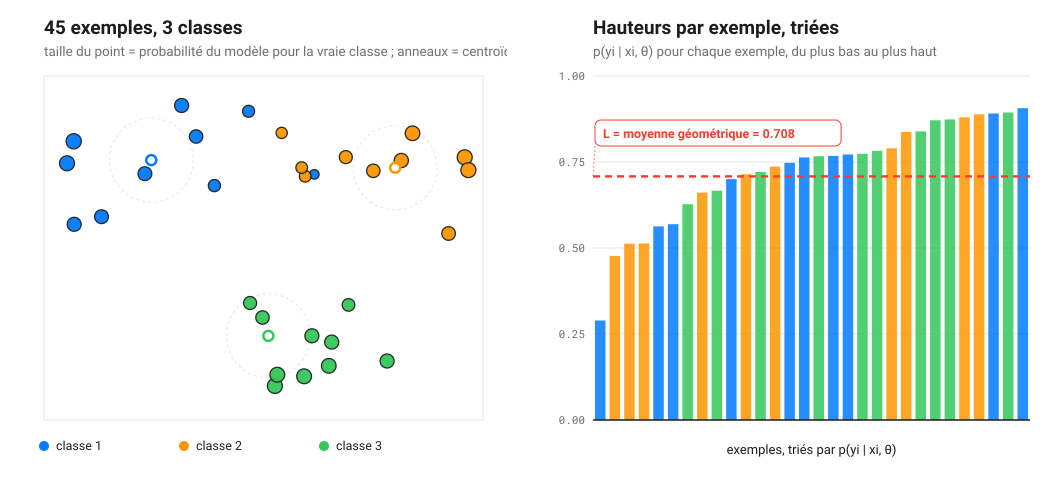
\includegraphics[width=\textwidth]{figures/classification_density_fr.png}
\caption{À gauche~: $45$ exemples simulés issus de $3$ classes qui se
chevauchent (les anneaux pointillés marquent les centroïdes
générateurs), la taille du point montrant la probabilité du modèle
pour la vraie classe propre à chaque exemple, petite près d'une
frontière de classe, grande profondément dans le territoire d'une
classe. À droite~: ces mêmes $45$ probabilités triées du plus bas au
plus haut, avec leur moyenne géométrique, le $L$ de cette note,
marquée.}
\label{fig:classification}
\end{figure}

Un simple scalaire, pourtant, que ce soit $\mathrm{CE}$,
$\exp(-\mathrm{CE})$ ou une perplexité, ne répond jamais qu'à «~à quel
point confiant, en moyenne~», jamais à «~à quelle fréquence
effectivement juste~». Un modèle peut se tromper avec assurance, en
attribuant une forte probabilité à une classe incorrecte. $\mathrm{CE}$
pénalise justement cet excès de confiance plus durement qu'une petite
incertitude honnête ne le serait, la même asymétrie qu'une règle de
score propre est construite pour avoir~: parier $99\,\%$ sur une classe
qui s'avère fausse coûte bien plus de nats que parier $60\,\%$ ne le
ferait jamais. Cette asymétrie, plus que le simple niveau de confiance
moyen, explique pourquoi c'est l'entropie croisée, et non l'exactitude
brute de classification, que la descente de gradient ajuste dans
pratiquement tout classifieur moderne.

\subsection{Régression sous bruit gaussien}
\label{sec:regression}

Soit $y_i = f(x_i;\theta) + \varepsilon_i$ avec $\varepsilon_i$ i.i.d.\
$\mathcal N(0,\sigma^2)$, $f$ une fonction de régression quelconque et
$\theta$ ses paramètres, la densité conditionnelle générique de la
section~\ref{sec:notion} spécialisée à une famille particulière~:

\begin{center}
\begin{tikzpicture}[
  node distance=13mm and 16mm,
  box/.style={draw, rounded corners, minimum height=8mm, minimum width=19mm,
    align=center, font=\small, fill=blue!4},
  sum/.style={draw, circle, minimum size=7mm, inner sep=0pt, font=\small},
  ->, >=Stealth, thick
]
\node[box] (theta) {$\theta$};
\node[box, right=of theta] (f) {$f(x_i;\theta)$};
\node[sum, right=of f] (sum) {$+$};
\node[box, right=of sum] (y) {$y_i$};
\node[box, below=of sum, fill=red!4] (eps) {$\varepsilon_i \sim \mathcal N(0,\sigma^2)$};
\draw (theta) -- (f);
\draw (f) -- (sum);
\draw (sum) -- (y);
\draw (eps) -- (sum);
\end{tikzpicture}
\end{center}

\begin{equation}
p(y_i \mid x_i, \theta) = (2\pi\sigma^2)^{-1/2}
\exp\!\left(-\frac{(y_i - f(x_i;\theta))^2}{2\sigma^2}\right)
\end{equation}

si bien que, en notant $\mathrm{MSE}(\theta) := \frac1n\sum_i (y_i -
f(x_i;\theta))^2$,

\begin{equation}
L(\theta,\sigma^2) = (2\pi\sigma^2)^{-1/2}\exp\!\left(-\frac{\mathrm{MSE}(\theta)}{2\sigma^2}\right).
\end{equation}

La figure~\ref{fig:regression} trace cette densité littéralement
plutôt qu'en simples symboles~: une petite cloche à quelques positions
$x$ choisies, chacune la densité conditionnelle $p(\cdot \mid
x_i,\theta)$ couchée sur le côté, sa largeur fixée par $\sigma$ et son
centre suivant la droite ajustée. Le point marqué sur chaque cloche
est la hauteur propre de cette courbe au point réellement observé,
$p(y_i \mid x_i,\theta)$, haute là où l'ajustement tombe près de la
donnée, basse sinon. $L$ n'est rien de plus que la moyenne géométrique
de ces hauteurs prise sur chaque observation, pas seulement les quatre
marquées, l'exact pendant continu des barres triées de la
figure~\ref{fig:classification}~: un ajustement proche presque partout
affiche surtout des hauteurs élevées et un $L$ grand, un ajustement
qui s'égare affiche quelques hauteurs basses qui tirent la moyenne
géométrique vers le bas, un mauvais écart faisant plus de dégâts sur
une moyenne géométrique que sur une moyenne arithmétique, la même
asymétrie que l'inégalité de Jensen de la section~\ref{sec:sens}
signalait déjà.

À la variance de maximum de vraisemblance $\hat\sigma^2 =
\mathrm{MSE}(\theta)$,

\begin{equation}
\exp(\mathbb E[\ln p]) = \frac{1}{\sqrt{2\pi e}\,\sqrt{\mathrm{MSE}(\theta)}},
\end{equation}

l'inverse de l'erreur quadratique moyenne racine à une constante
universelle $\sqrt{2\pi e}$ près, l'exact pendant continu de la
lecture inverse-perplexité de la section~\ref{sec:classification}~:
dans les deux cas, $\exp(\mathbb E[\ln p])$ est l'inverse d'une mesure
d'erreur propre à la tâche de prédiction, la perplexité pour une
prédiction catégorielle, l'erreur quadratique moyenne racine pour une
prédiction continue. Ce n'est pas une coïncidence. En notant $\ell :=
\ln L$ et, suivant la convention des critères d'information,
$\mathrm{PPL} := \exp(-2\ell)$, l'identité $\exp(\mathbb E[\ln p]) =
1/\sqrt{\mathrm{PPL}}$ tient en général, que le modèle soit gaussien ou
non, une conséquence directe des deux définitions plutôt qu'une
propriété propre à l'un ou l'autre cas travaillé. La propre
\code{ELBOW-fr.tex} d'\code{elbow-helper} pousse cette instanciation
plus loin~: $f$ y parcourt les droites simples, les lignes brisées et
les lignes brisées à $k$ segments. Le $\mathrm{PPL}$ y devient un
score véritablement borné et ancré sur un pire cas, plutôt que laissé
comme une simple lecture inverse-RMSE.

\begin{figure}[H]
\centering
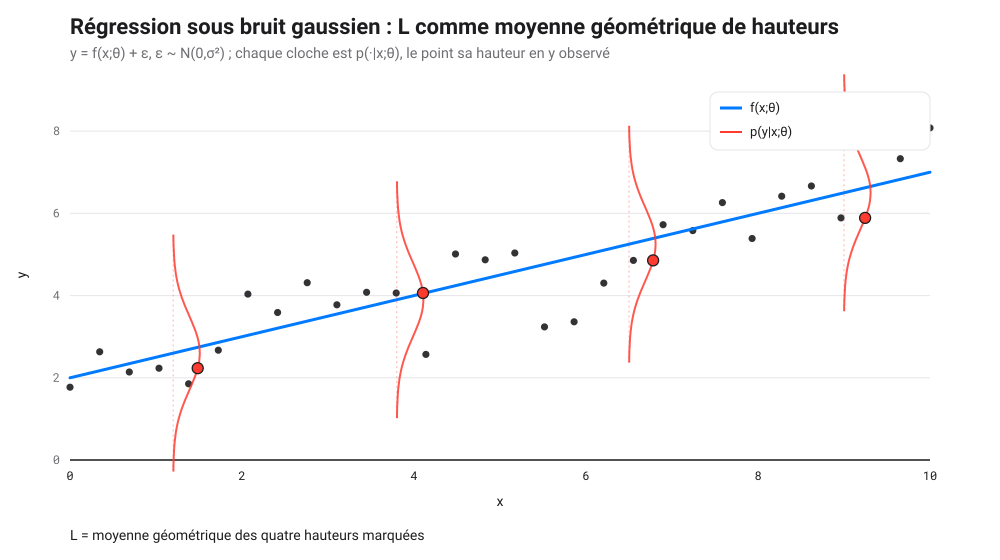
\includegraphics[width=\textwidth]{figures/regression_density_fr.png}
\caption{Données de régression synthétiques, $y = 2 + 0{,}5x +
\varepsilon$, $\varepsilon \sim \mathcal N(0, 0{,}9^2)$, avec la droite
ajustée et quatre courbes de densité conditionnelle $p(\cdot \mid
x,\theta)$ tracées à des positions $x$ choisies. Chaque point marque
la hauteur propre de cette courbe à la valeur réellement observée là.
$L$ est la moyenne géométrique de chaque hauteur, pas seulement les
quatre marquées~: haute là où l'ajustement tombe près de la donnée,
basse là où un point s'éloigne du centre de la courbe.}
\label{fig:regression}
\end{figure}

\section{Une conclusion pratique~: borner la vraisemblance}
\label{sec:conclusion}

Chaque quantité que cette note a construite, $\mathrm{CE}$, $\ell$,
$\mathrm{PPL}$, est une remise à l'échelle du même nombre sous-jacent.
Chacune de ces remises à l'échelle partage le même premier problème~:
prise brute, elle n'a pas de plafond, si bien qu'aucun seuil unique
dessus ne signifie la même chose d'un ajustement à l'autre. Y remédier
demande de s'ancrer contre un pire cas réel et atteignable plutôt que
contre un cas arbitraire ou inaccessible, un geste que la
classification ne doit faire qu'une fois et que la régression doit
faire deux fois, pour une raison qui mérite d'être précisée plutôt que
simplement évoquée.

Le $\mathrm{CE}(\theta) \ge 0$ de la classification a déjà un plancher
propre~: nul exactement pour une prédiction parfaitement confiante et
correcte, rien de spécial à faire pour l'atteindre. Le balayage en
température de la section~\ref{sec:sens} a déjà nommé le plafond
naturel contre lequel s'ancrer. Quand $\beta \to 0$, chaud et
maximalement agité, la confiance de n'importe quel modèle s'aplatit
vers l'uniforme sur les $K$ classes, indépendamment de ce qu'il croyait
réellement. Un modèle qui prédit uniformément obtient exactement
$\mathrm{CE} = \ln K$ sur n'importe quelle vraie classe, la seule
valeur d'entropie croisée qui ne dépend pas de la classe qui s'avère
juste. Ce n'est pas une référence arbitraire~: c'est ce que coûte, en
nats, le refus d'utiliser la moindre information propre au modèle,
quelle que soit l'étiquette, si bien que
$$Q_{\text{classif}}(\theta) := 1 - \frac{\mathrm{CE}(\theta)}{\ln K}$$
vaut $1$ pour un modèle parfaitement confiant et correct, $0$ pour un
modèle qui ne vaut pas mieux qu'un tirage uniforme, et une valeur
négative pour un modèle activement trompeur, confiant à tort plus
souvent que confiant à raison, un signal que cette note ne voit aucune
raison de masquer en l'écrêtant.

La log-vraisemblance propre à la régression n'a pas un tel plancher.
C'est le second problème, distinct du plafond que les deux cas
partagent. Une densité continue peut dépasser $1$, si bien que profiler
$\sigma^2$ à sa valeur la mieux soutenue $\hat\sigma^2 =
\mathrm{MSE}(\theta)$ envoie $\ell(\theta,\hat\sigma^2)$ vers $+\infty$,
pas vers un $0$ propre, exactement à l'ajustement parfait, la
dégénérescence classique de la vraisemblance qui justifie l'existence
même du BIC. Exponentier répare d'abord cela~: $\mathrm{PPL}(\theta) :=
\exp(-2\ell(\theta,\hat\sigma^2)) = 2\pi e \cdot \mathrm{MSE}(\theta)
\ge 0$, nul exactement à l'ajustement parfait, toujours non borné
au-dessus mais partant désormais d'un plancher sur lequel construire.
La propre \code{ELBOW-fr.tex} d'\code{elbow-helper} fournit le second
geste, le plafond~: non une formule mais un véritable pire cas tiré des
données elles-mêmes, le seul point \emph{observé} $y_{\text{bad}}$ le
plus difficile à partir duquel prédire tous les autres, donnant à
$\mathrm{MSE}_{\text{worst}}$ exactement le rôle que joue $\ln K$
ci-dessus,
$$Q_{\text{reg}}(\theta) := 1 - \frac{\mathrm{MSE}(\theta)}{\mathrm{MSE}_{\text{worst}}} = 1 - \frac{\mathrm{PPL}(\theta)}{\mathrm{PPL}_{\text{worst}}},$$
les deux rapports étant égaux parce que $\mathrm{PPL}$ et
$\mathrm{MSE}$ portent la même constante $2\pi e$ au numérateur comme
au dénominateur.

Deux pires cas différents répondent à la même question dans les deux
seules façons que permet le modèle génératif propre à cette note. Un
classifieur à $K$ catégories a une alternative fixe, indépendante de
l'étiquette, intégrée à sa propre structure, le tirage uniforme, et
n'a jamais besoin de regarder les données pour en trouver une. Un
régresseur continu n'a pas une telle alternative intégrée~: rien dans
la famille du modèle seule ne dit à quoi ressemble une mauvaise
prédiction, si bien que le pire cas doit être emprunté à l'échantillon
même que le modèle essaie d'ajuster. Une fois cette asymétrie prise en
compte plutôt que masquée, $\mathrm{CE}$ et $\mathrm{MSE}$, des nombres
qui n'avaient de sens que face à une autre exécution du même modèle sur
les mêmes données, deviennent $Q_{\text{classif}}$ et $Q_{\text{reg}}$,
des nombres qui signifient la même chose sur n'importe quel jeu de
données, de n'importe quelle taille, dans l'une ou l'autre langue dans
laquelle cette note est écrite.

\clearpage

\bibliography{references}

\end{document}
